%\title{LaTeX Portrait Poster Template}
%%%%%%%%%%%%%%%%%%%%%%%%%%%%%%%%%%%%%%%%%
% a0poster Portrait Poster
% LaTeX Template
% Version 1.0 (22/06/13)
%
% The a0poster class was created by:
% Gerlinde Kettl and Matthias Weiser (tex@kettl.de)
% 
% Adapter by Jens Buysse for Hogeschool Gent
% This template has been downloaded from:
% http://www.LaTeXTemplates.com
%
% License:
% CC BY-NC-SA 3.0 (http://creativecommons.org/licenses/by-nc-sa/3.0/)
%
%%%%%%%%%%%%%%%%%%%%%%%%%%%%%%%%%%%%%%%%%

%----------------------------------------------------------------------------------------
%	PACKAGES AND OTHER DOCUMENT CONFIGURATIONS
%----------------------------------------------------------------------------------------

\documentclass[a0,portrait]{a0poster}

\usepackage{multicol} % This is so we can have multiple columns of text side-by-side
\columnsep=100pt % This is the amount of white space between the columns in the poster
\columnseprule=3pt % This is the thickness of the black line between the columns in the poster

\usepackage[svgnames]{xcolor} % Specify colors by their 'svgnames', for a full list of all colors available see here: http://www.latextemplates.com/svgnames-colors

\usepackage{times} % Use the times font
%\usepackage{palatino} % Uncomment to use the Palatino font

\usepackage{graphicx} % Required for including images
\graphicspath{{figures/}} % Location of the graphics files
\usepackage{booktabs} % Top and bottom rules for table
\usepackage[font=small,labelfont=bf]{caption} % Required for specifying captions to tables and figures
\usepackage{amsfonts, amsmath, amsthm, amssymb} % For math fonts, symbols and environments
\usepackage{wrapfig} % Allows wrapping text around tables and figures
\usepackage[export]{adjustbox}

\begin{document}

%----------------------------------------------------------------------------------------
%	POSTER HEADER 
%----------------------------------------------------------------------------------------

% The header is divided into two boxes:
% The first is 75% wide and houses the title, subtitle, names, university/organization and contact information
% The second is 25% wide and houses a logo for your university/organization or a photo of you
% The widths of these boxes can be easily edited to accommodate your content as you see fit

\begin{minipage}[t]{0.75\linewidth}
\VeryHuge \color{HoGentAccent1} \textbf{A secure environment for conducting examinations on personal devices} \color{Black}\\ % Title
\Huge\textit{}\\[2.4cm] % Subtitle
\huge \textbf{Viaene Kjell, Dhr. Van Vreckem Bert, Mevr. De Donder Margot}\\[0.5cm] % Author(s)
\huge Hogeschool Gent, Valentin Vaerwyckweg 1, 9000 Gent\\[0.4cm] % University/organization
\Large \texttt{kjell.viaene.v7322@student.hogent.be} \\
\end{minipage}
%
\begin{minipage}[t]{0.25\linewidth}

\includegraphics[width=13cm,right]{figures/HG-woordmerk.jpg} 

\end{minipage}

\vspace{1cm} % A bit of extra whitespace between the header and poster content

%----------------------------------------------------------------------------------------

\begin{multicols}{2} % This is how many columns your poster will be broken into, a portrait poster is generally split into 2 columns

%----------------------------------------------------------------------------------------
%	ABSTRACT
%----------------------------------------------------------------------------------------

\color{HoGentAccent1} % Navy color for the abstract

\begin{abstract}
Setting up a secure environment in any environment is a challenge. With technology constantly chancing, especially in the IT sector, it's always hard to keep security up to date. The core purpose of this thesis is to build a system that ensures students who are taking part in a digital examination only have access to those resources which they are allowed to use. \\ Having a system like this is crucial to having a good grading system. And to minimize the chances that a student cheated. When students are able to cheat at examinations as easily as they often can now, all the value of an examination is lost.\\ For the school itself it might seem like the course is too easy and needs to be made more difficult. Which can have a bad effect on the course as a whole. This might result in the students thinking that the course is no challenge and will pass the exam without any real knowledge of the subject. This may come back to bite them (follow up courses, job interviews, ...).
Multiple methods were tested to find a system in which these problems are resolved. These methods are:
\begin{itemize}
\item Filtering using a DNS Whitelist
\item Filtering using an ACL on a router
\item Filtering using a firewall
\item Filtering using an application.
\end{itemize}
These are the most common ways of filtering internet access in a network. Research is done as to what method is good and how good these methods are compared with each other. How complicated they are to set up and maintain. After testing these methods a conclusion was made that DNS whitelisting is the worst choice. This method requires the most work and has the lowest performance/quality rating. The router ACL method and setting up a firewall are pretty matching in performance and quality. They are easy to configure and allow for better protection. The firewall has more possibilities but can be harder to set up while the router is a bit simpler but is easy to set up. The best choice however is without a doubt the application (Safe Exam Browser). This application secures every device on its own and allows for local filtering of the internet and the local files. This is the perfect solution to our issue. It's easy to use and performs really well. The only downside to it is that there is no integration with Chamilo. It can still be used but some authorization methods are not applicable. This however could be the subject of an other research paper.
\end{abstract}
%----------------------------------------------------------------------------------------
%	INTRODUCTION
%----------------------------------------------------------------------------------------
\color{HoGentAccent1} 
\section*{Introduction}
\color{black}
\color{black}
At present, a lot of schools (including the HoGent) struggle with setting up environments in which digital examinations can be conducted. This often occurs because of the lack of knowledge around IT or around the general possibilities there are. There are multiple ways to do this and it might not always be clear what way is the one to take. Certain advantages and disadvantage  of those methods are not known as well. That's why in this thesis the most commonly known ways of setting up such an environment are tested and compared with each other. When the thesis has been read the reader will be able to determine what solution fits his needs the best. While also understanding the multiple ways that are viable options. 
\\
The objective of this thesis is to be able to start with an unprotected environment and to be able to make a protected one out of it. While taking into account the scenarios in which the environment is located. If a way is found to protect the environment in multiple ways we can see the objective as reached. If however the conclusion is that no method really fulfills our needs, then this thesis has failed its purpose. But even then there will be more clarity around the possible ways of filtering data in a network.
The most important task to complete in this thesis is to find a solution to our problem. This solution has to be of a certain difficulty level that is not to high as we want it to be easy implementable and understandable. This way not only IT professionals would be able to use it. 
\begin{center}\vspace{1cm}
\captionof{figure}{\color{HoGentAccent5} All tested methods are evaluated on each of the mentioned criteria.}
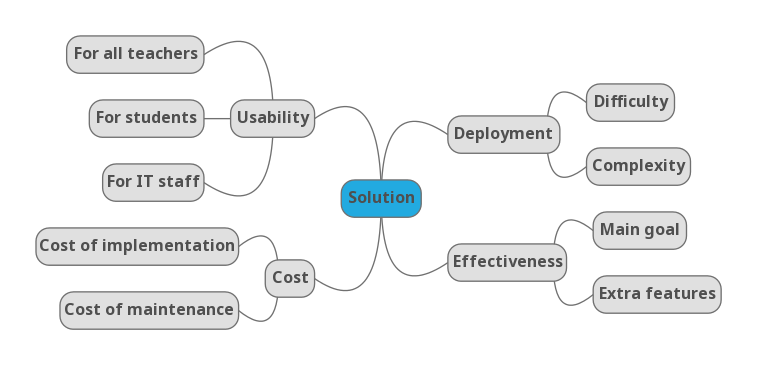
\includegraphics[width=1.0\linewidth]{mindmap}
\end{center}
%----------------------------------------------------------------------------------------
%	GEOLOGY
%----------------------------------------------------------------------------------------

\color{Black} % DarkSlateGray color for the rest of the content
\color{HoGentAccent1} 
\section*{Testing}
\color{black}
In order to test all mentioned methods a test environment was build. This was achieved by using virtual machines which each symbolized a physical network device. During these tests a conclusion was made for each method as to how far they met the criteria. The firewall was only implemented when tested. In all other cases the servers were directly connected with the router, as was the user.

\begin{center}\vspace{1cm}
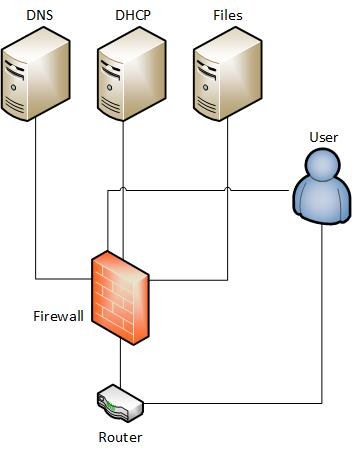
\includegraphics[scale=2]{environment}
\captionof{figure}{\color{HoGentAccent5} The test environment used in this thesis. The setup was automated by using vagrant.}
\end{center}\vspace{1cm}

%------------------------------------------------



\color{HoGentAccent1} 
\section*{Conclusions}
\color{black}
After testing all proposed solutions a clear winner was selected. This being \textit{filtering by using an application}. The application that was tested was Safe Exam Browser\footnote{https://www.safeexambrowser.org/}. This application allowed us to reach the set goal of filtering unwanted websites. But it added a lot more features that were not even requested. The implementation is incredibly easy and can be performed by people without any real IT knowledge. It allows schools to monitor the use of a persons personal device while not having to monitor their system live and breaking possible privacy laws.\\
From the other tested methods the DNS is the big loser. Being hard to implement and not as effective as a router or firewall it ends on the last place. The router and firewall share a second place. The first being faster to deploy while the second being a bit more broader in possibilities.
%----------------------------------------------------------------------------------------
%	FORTHCOMING RESEARCH
%----------------------------------------------------------------------------------------
\color{HoGentAccent1} 
\section*{Future research}
\color{black}
The integration of SEB into Chamilo would be interesting to further investigate. It would
make the lives of teachers a lot easier in our school. Maybe it can be made so that SEB
is actually installed on a server in the school and that the students boot it via that server
and this way it might add an extra layer of protection. Research into the other methods
seems kind of a waste of time as it is clear that there are way more modern and better
choices on the market that do much more. The only things that might be interesting is to
find a way to effectively find correct IP-Addresses, for certain domains which you want
to block, that keeps being up to date. So basically, automating the set-up of a dynamic
whitelist.


%----------------------------------------------------------------------------------------

\end{multicols}
\end{document}